\documentclass[14pt]{extbook}
\usepackage{multicol, enumerate, enumitem, hyperref, color, soul, setspace, parskip, fancyhdr} %General Packages
\usepackage{amssymb, amsthm, amsmath, latexsym, units, mathtools} %Math Packages
\everymath{\displaystyle} %All math in Display Style
% Packages with additional options
\usepackage[headsep=0.5cm,headheight=12pt, left=1 in,right= 1 in,top= 1 in,bottom= 1 in]{geometry}
\usepackage[usenames,dvipsnames]{xcolor}
\usepackage{dashrule}  % Package to use the command below to create lines between items
\newcommand{\litem}[1]{\item#1\hspace*{-1cm}\rule{\textwidth}{0.4pt}}
\pagestyle{fancy}
\lhead{Progress Quiz 2}
\chead{}
\rhead{Version C}
\lfoot{4389-3341}
\cfoot{}
\rfoot{Summer C 2021}
\begin{document}

\begin{enumerate}
\litem{
Find the equation of the line described below. Write the linear equation in the form $ y=mx+b $ and choose the intervals that contain $m$ and $b$.\[ \text{Perpendicular to } 8 x - 7 y = 9 \text{ and passing through the point } (-5, -10). \]\begin{enumerate}[label=\Alph*.]
\item \( m \in [0.58, 0.96] \hspace*{3mm} b \in [-5.8, -5.1] \)
\item \( m \in [-1.61, -1.05] \hspace*{3mm} b \in [-16.4, -11.7] \)
\item \( m \in [-0.99, -0.78] \hspace*{3mm} b \in [-5.3, -4.9] \)
\item \( m \in [-0.99, -0.78] \hspace*{3mm} b \in [11.9, 14.4] \)
\item \( m \in [-0.99, -0.78] \hspace*{3mm} b \in [-16.4, -11.7] \)

\end{enumerate} }
\litem{
Solve the equation below. Then, choose the interval that contains the solution.\[ -15(-6x + 19) = -14(12x + 4) \]\begin{enumerate}[label=\Alph*.]
\item \( x \in [-4.6, -4.26] \)
\item \( x \in [0.94, 1.57] \)
\item \( x \in [0.34, 1.31] \)
\item \( x \in [-1.67, -0.74] \)
\item \( \text{There are no real solutions.} \)

\end{enumerate} }
\litem{
Solve the equation below. Then, choose the interval that contains the solution.\[ -16(4x + 7) = -11(13x + 5) \]\begin{enumerate}[label=\Alph*.]
\item \( x \in [-1.4, 0.2] \)
\item \( x \in [1, 2.5] \)
\item \( x \in [-0.8, 1.2] \)
\item \( x \in [-2.5, -2] \)
\item \( \text{There are no real solutions.} \)

\end{enumerate} }
\litem{
Write the equation of the line in the graph below in Standard Form $Ax+By=C$. Then, choose the intervals that contain $A, B, \text{ and } C$.
\begin{center}
    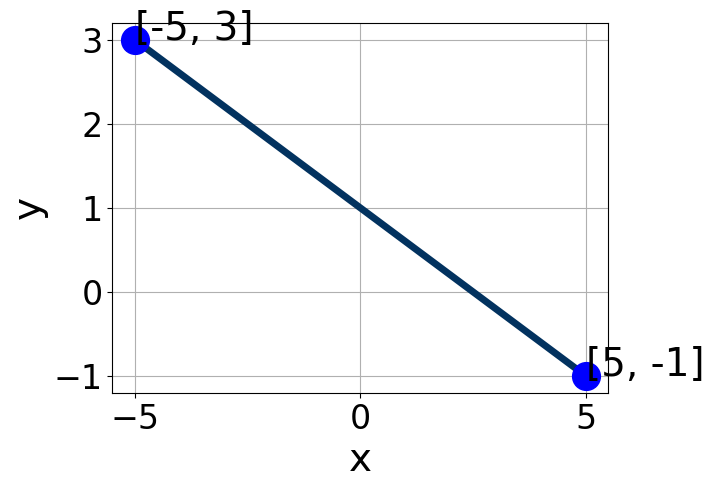
\includegraphics[width=0.5\textwidth]{../Figures/linearGraphToStandardCopyC.png}
\end{center}
\begin{enumerate}[label=\Alph*.]
\item \( A \in [-3.5, -0.3], \hspace{3mm} B \in [-6.5, -4.5], \text{ and } \hspace{3mm} C \in [-5.8, -1.4] \)
\item \( A \in [1.9, 3.7], \hspace{3mm} B \in [-6.5, -4.5], \text{ and } \hspace{3mm} C \in [-5.8, -1.4] \)
\item \( A \in [1.9, 3.7], \hspace{3mm} B \in [2.5, 6], \text{ and } \hspace{3mm} C \in [4.7, 8.4] \)
\item \( A \in [-0.4, 0.7], \hspace{3mm} B \in [0.2, 1.1], \text{ and } \hspace{3mm} C \in [-0.4, 3.2] \)
\item \( A \in [-0.4, 0.7], \hspace{3mm} B \in [-1.9, 0.5], \text{ and } \hspace{3mm} C \in [-2.4, -0.8] \)

\end{enumerate} }
\litem{
Solve the linear equation below. Then, choose the interval that contains the solution.\[ \frac{-3x -3}{2} - \frac{-7x + 6}{3} = \frac{7x -4}{8} \]\begin{enumerate}[label=\Alph*.]
\item \( x \in [-3, 1] \)
\item \( x \in [23, 29] \)
\item \( x \in [-74, -67] \)
\item \( x \in [-126, -119] \)
\item \( \text{There are no real solutions.} \)

\end{enumerate} }
\litem{
Find the equation of the line described below. Write the linear equation in the form $ y=mx+b $ and choose the intervals that contain $m$ and $b$.\[ \text{Perpendicular to } 8 x - 3 y = 7 \text{ and passing through the point } (10, -9). \]\begin{enumerate}[label=\Alph*.]
\item \( m \in [-0.16, 0.45] \hspace*{3mm} b \in [-15.75, -9.75] \)
\item \( m \in [-0.49, -0.3] \hspace*{3mm} b \in [3.25, 8.25] \)
\item \( m \in [-3.16, -2.5] \hspace*{3mm} b \in [-6.25, -1.25] \)
\item \( m \in [-0.49, -0.3] \hspace*{3mm} b \in [-21, -17] \)
\item \( m \in [-0.49, -0.3] \hspace*{3mm} b \in [-6.25, -1.25] \)

\end{enumerate} }
\litem{
Solve the linear equation below. Then, choose the interval that contains the solution.\[ \frac{-4x -9}{4} - \frac{5x -7}{6} = \frac{-5x + 8}{7} \]\begin{enumerate}[label=\Alph*.]
\item \( x \in [-1.5, 0.7] \)
\item \( x \in [-4.8, -2.6] \)
\item \( x \in [-3, -1.3] \)
\item \( x \in [-9.5, -7.7] \)
\item \( \text{There are no real solutions.} \)

\end{enumerate} }
\litem{
First, find the equation of the line containing the two points below. Then, write the equation in the form $ y=mx+b $ and choose the intervals that contain $m$ and $b$.\[ (8, 11) \text{ and } (7, -3) \]\begin{enumerate}[label=\Alph*.]
\item \( m \in [9, 15] \hspace*{3mm} b \in [3, 8] \)
\item \( m \in [9, 15] \hspace*{3mm} b \in [-10, -7] \)
\item \( m \in [-18, -9] \hspace*{3mm} b \in [94, 97] \)
\item \( m \in [9, 15] \hspace*{3mm} b \in [-101, -95] \)
\item \( m \in [9, 15] \hspace*{3mm} b \in [101, 103] \)

\end{enumerate} }
\litem{
Write the equation of the line in the graph below in Standard Form $Ax+By=C$. Then, choose the intervals that contain $A, B, \text{ and } C$.
\begin{center}
    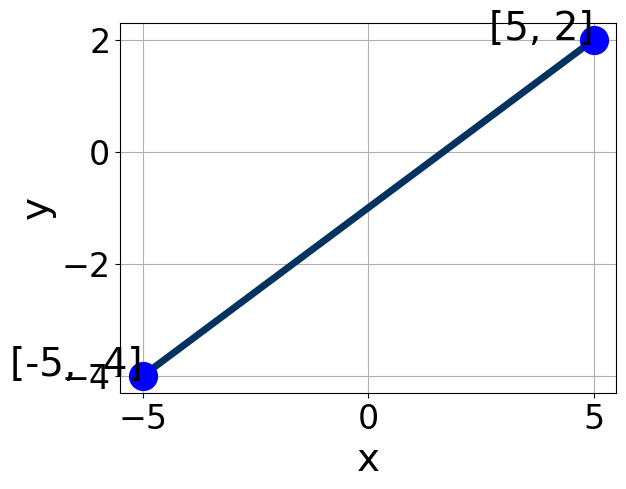
\includegraphics[width=0.5\textwidth]{../Figures/linearGraphToStandardC.png}
\end{center}
\begin{enumerate}[label=\Alph*.]
\item \( A \in [1.4, 6.1], \hspace{3mm} B \in [-5.4, -3.64], \text{ and } \hspace{3mm} C \in [3.4, 8.8] \)
\item \( A \in [-3.6, -2.4], \hspace{3mm} B \in [4.83, 5.33], \text{ and } \hspace{3mm} C \in [-7.3, -4.3] \)
\item \( A \in [-1.6, -0.5], \hspace{3mm} B \in [0.66, 1.66], \text{ and } \hspace{3mm} C \in [-2, -0.8] \)
\item \( A \in [1.4, 6.1], \hspace{3mm} B \in [4.83, 5.33], \text{ and } \hspace{3mm} C \in [-7.3, -4.3] \)
\item \( A \in [-1.6, -0.5], \hspace{3mm} B \in [-2.39, -0.89], \text{ and } \hspace{3mm} C \in [-0.7, 4.8] \)

\end{enumerate} }
\litem{
First, find the equation of the line containing the two points below. Then, write the equation in the form $ y=mx+b $ and choose the intervals that contain $m$ and $b$.\[ (-8, 11) \text{ and } (10, -5) \]\begin{enumerate}[label=\Alph*.]
\item \( m \in [0.5, 1.8] \hspace*{3mm} b \in [-14.8, -12.7] \)
\item \( m \in [-3.7, 0.5] \hspace*{3mm} b \in [1.6, 6.1] \)
\item \( m \in [-3.7, 0.5] \hspace*{3mm} b \in [-16, -14.5] \)
\item \( m \in [-3.7, 0.5] \hspace*{3mm} b \in [17.8, 21] \)
\item \( m \in [-3.7, 0.5] \hspace*{3mm} b \in [-4.4, -1.9] \)

\end{enumerate} }
\end{enumerate}

\end{document}